\section*{Divergence and anomalies for $\bf\alpha=-\frac{1}{3}$ at $\bf\Delta t = 0.01s$}
An interesting observation that can be made with regards to the case of $\alpha = -1/3$ is that if the algorithm is run long enough times it diverges. This can be attributed to the fact that the $\beta$ and $\gamma$ values do not ensure unconditional stability. The following plots verify proposition. 
\subsection*{No Body force}
\begin{itemize}
\item {\bf Stress-Strain Time Histories} 
\begin{center}
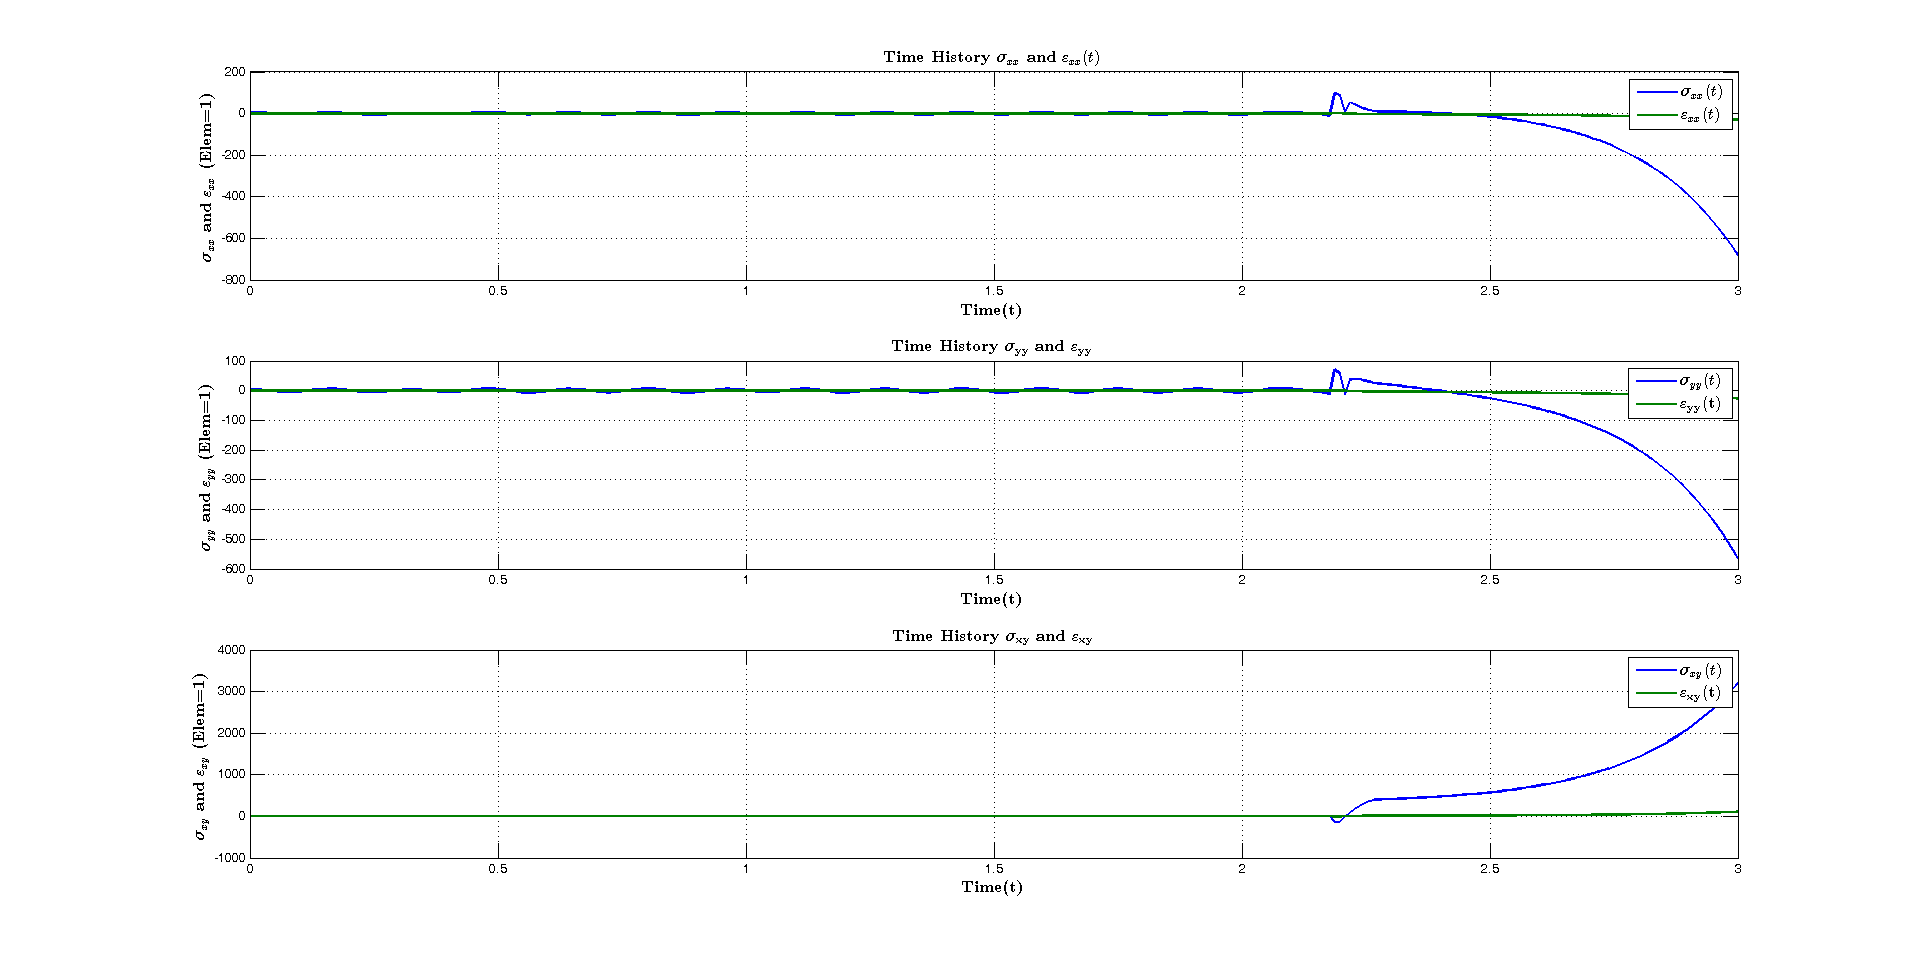
\includegraphics[height=5.5in,width=7in]{Sress_nobf_alphm1_3_b}
\end{center}\hrule
\item {\bf Comments: } The stresses and strains, in all components diverge after a certain point. This is due to the loss of stability and energy anomaly observed on the next page. 
\newpage
\item {\bf Displacement and Energy Time Histories}
\begin{center}
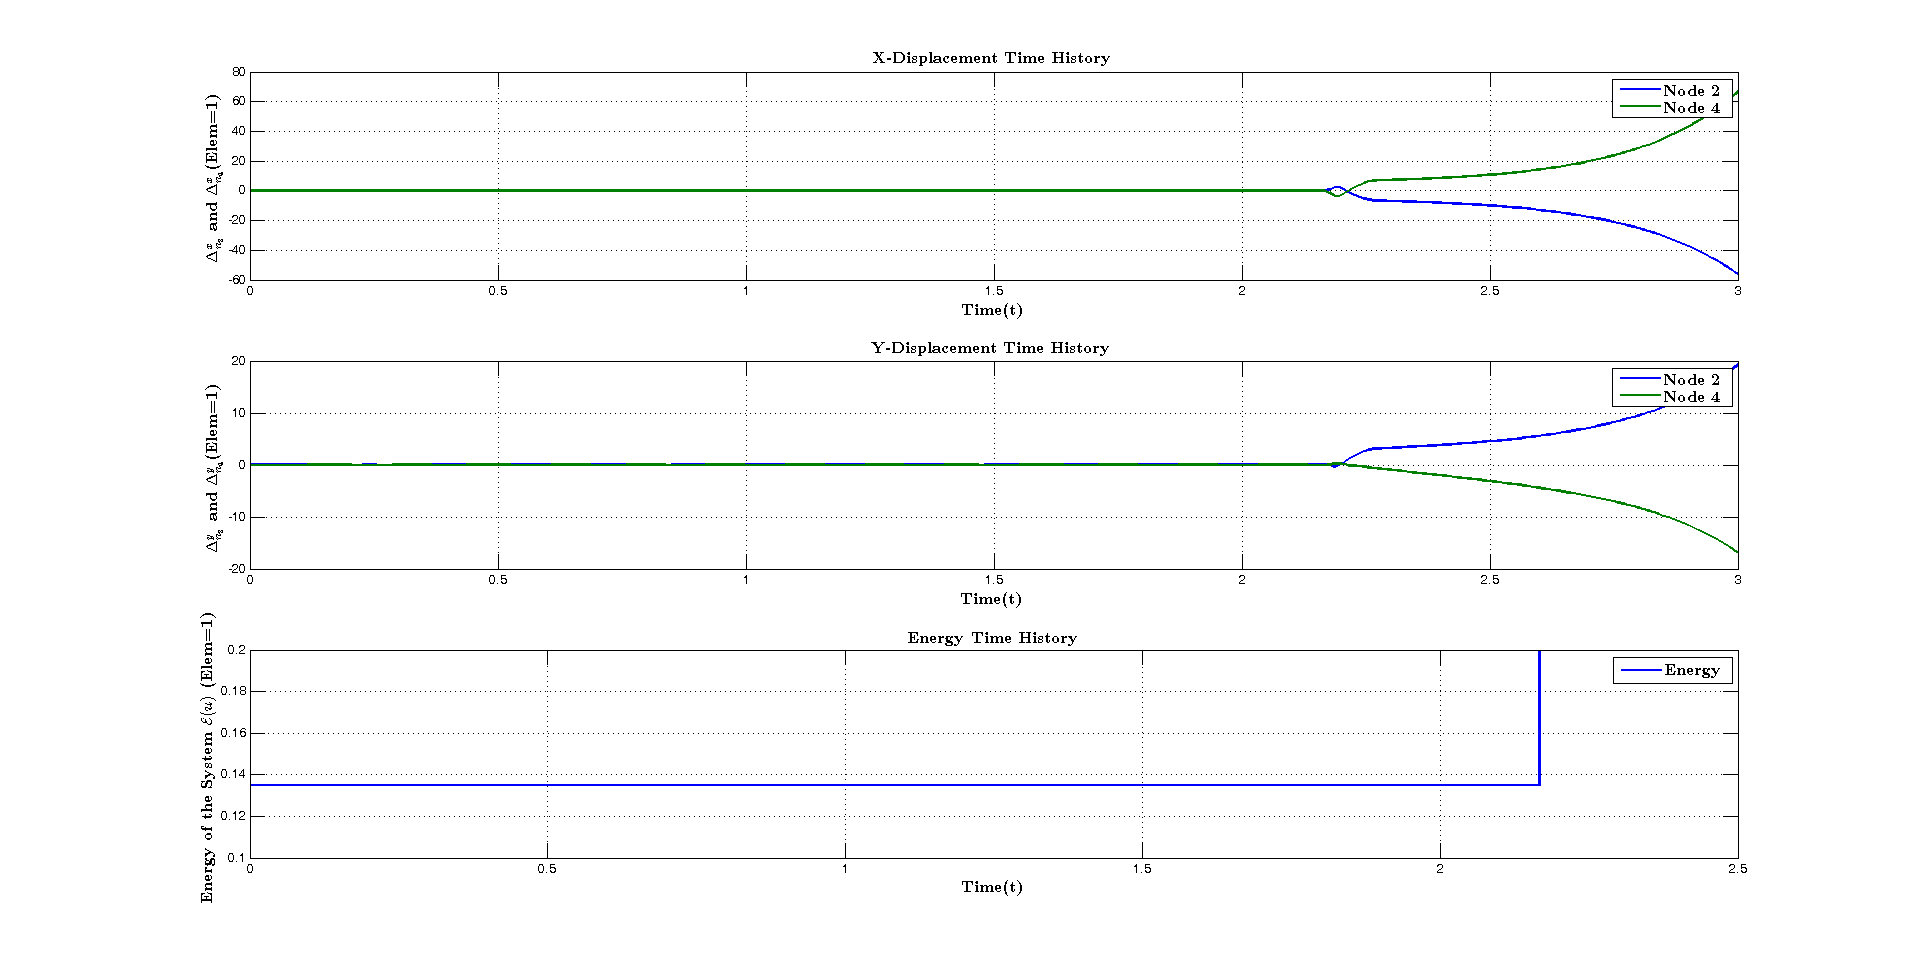
\includegraphics[height=5.5in,width=7in]{Disp_nobf_alphm1_3_b}
\end{center}\hrule
\item {\bf Comments: } The energy of the system blows up at a particular time instant as observed above which eventually leads to divergence. The following section illustrates that this problem is overcome when the system is resolved to a finer time increment, $\Delta t = 0.001s$, but in principle even that is not an unconditionally stable case. 
\newpage
\item {\bf Stress-Strain Time Histories $\bf\Delta t = 0.001s$} 
\begin{center}
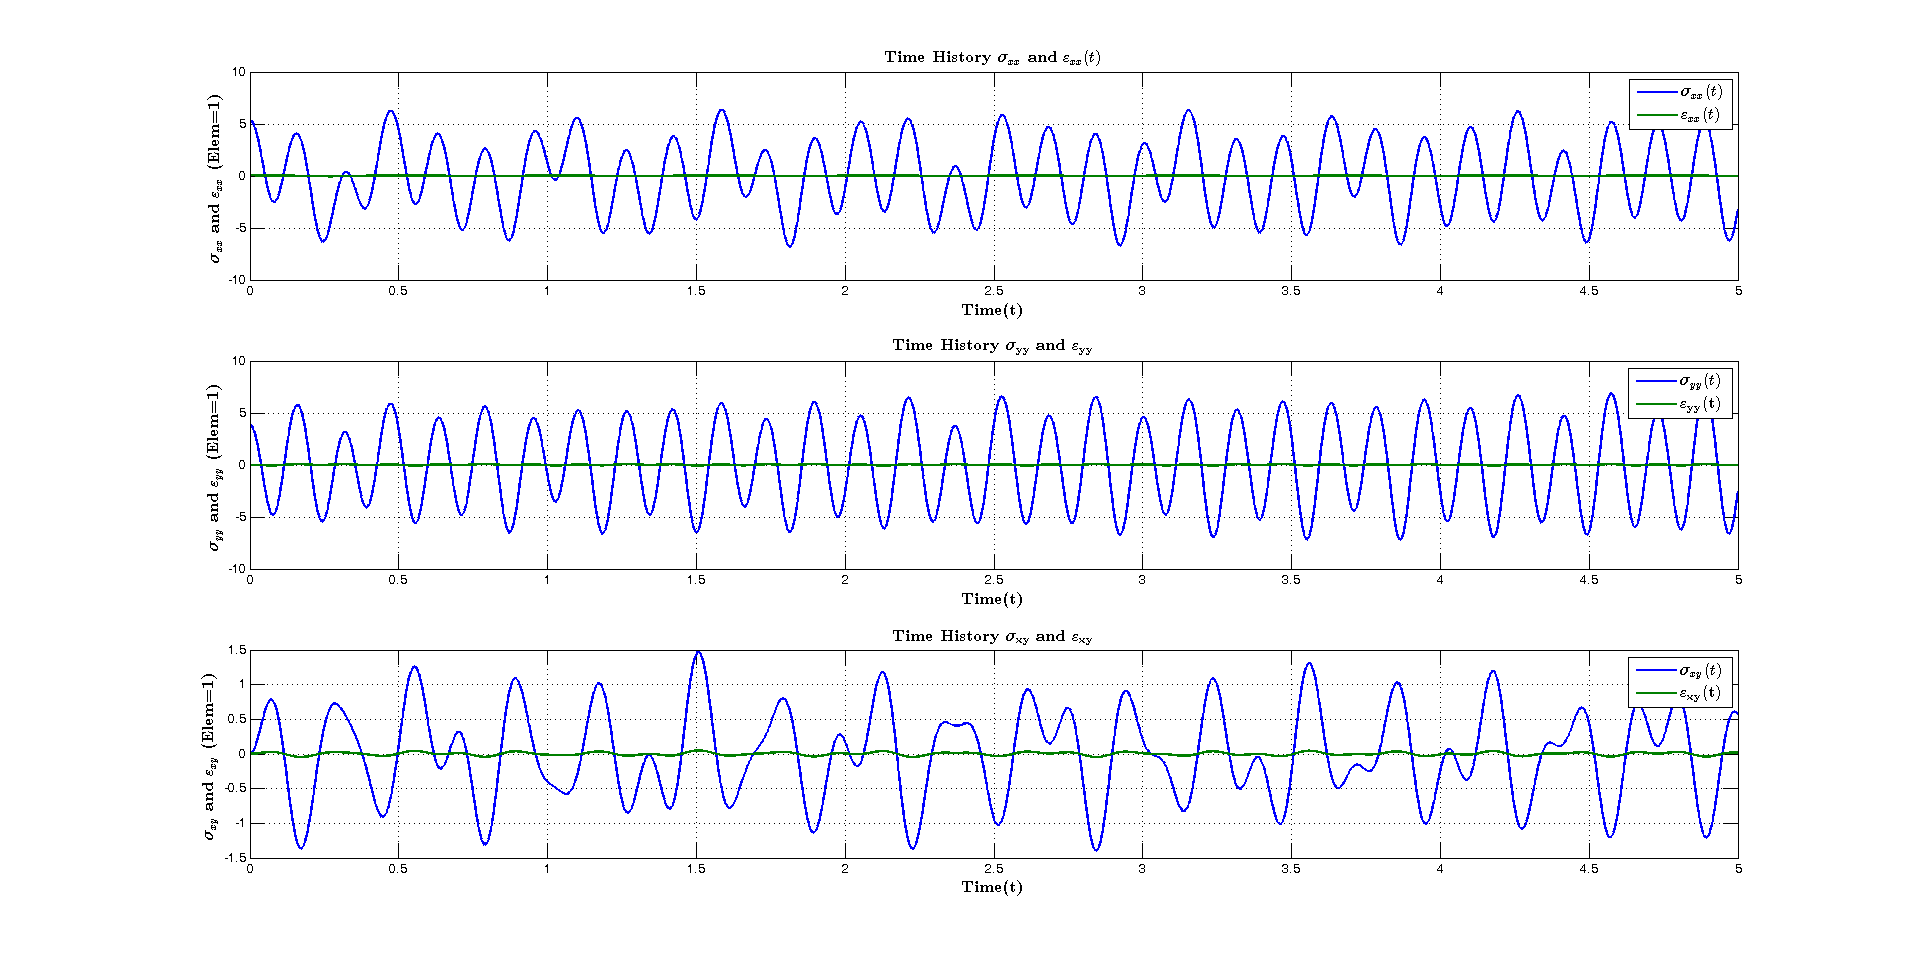
\includegraphics[height=5.5in,width=5.5in]{Sress_nobf_alphm1_3t3}
\end{center}\hrule 
\end{itemize}
\newpage {\bf And similarly for displacements} 
\begin{center}
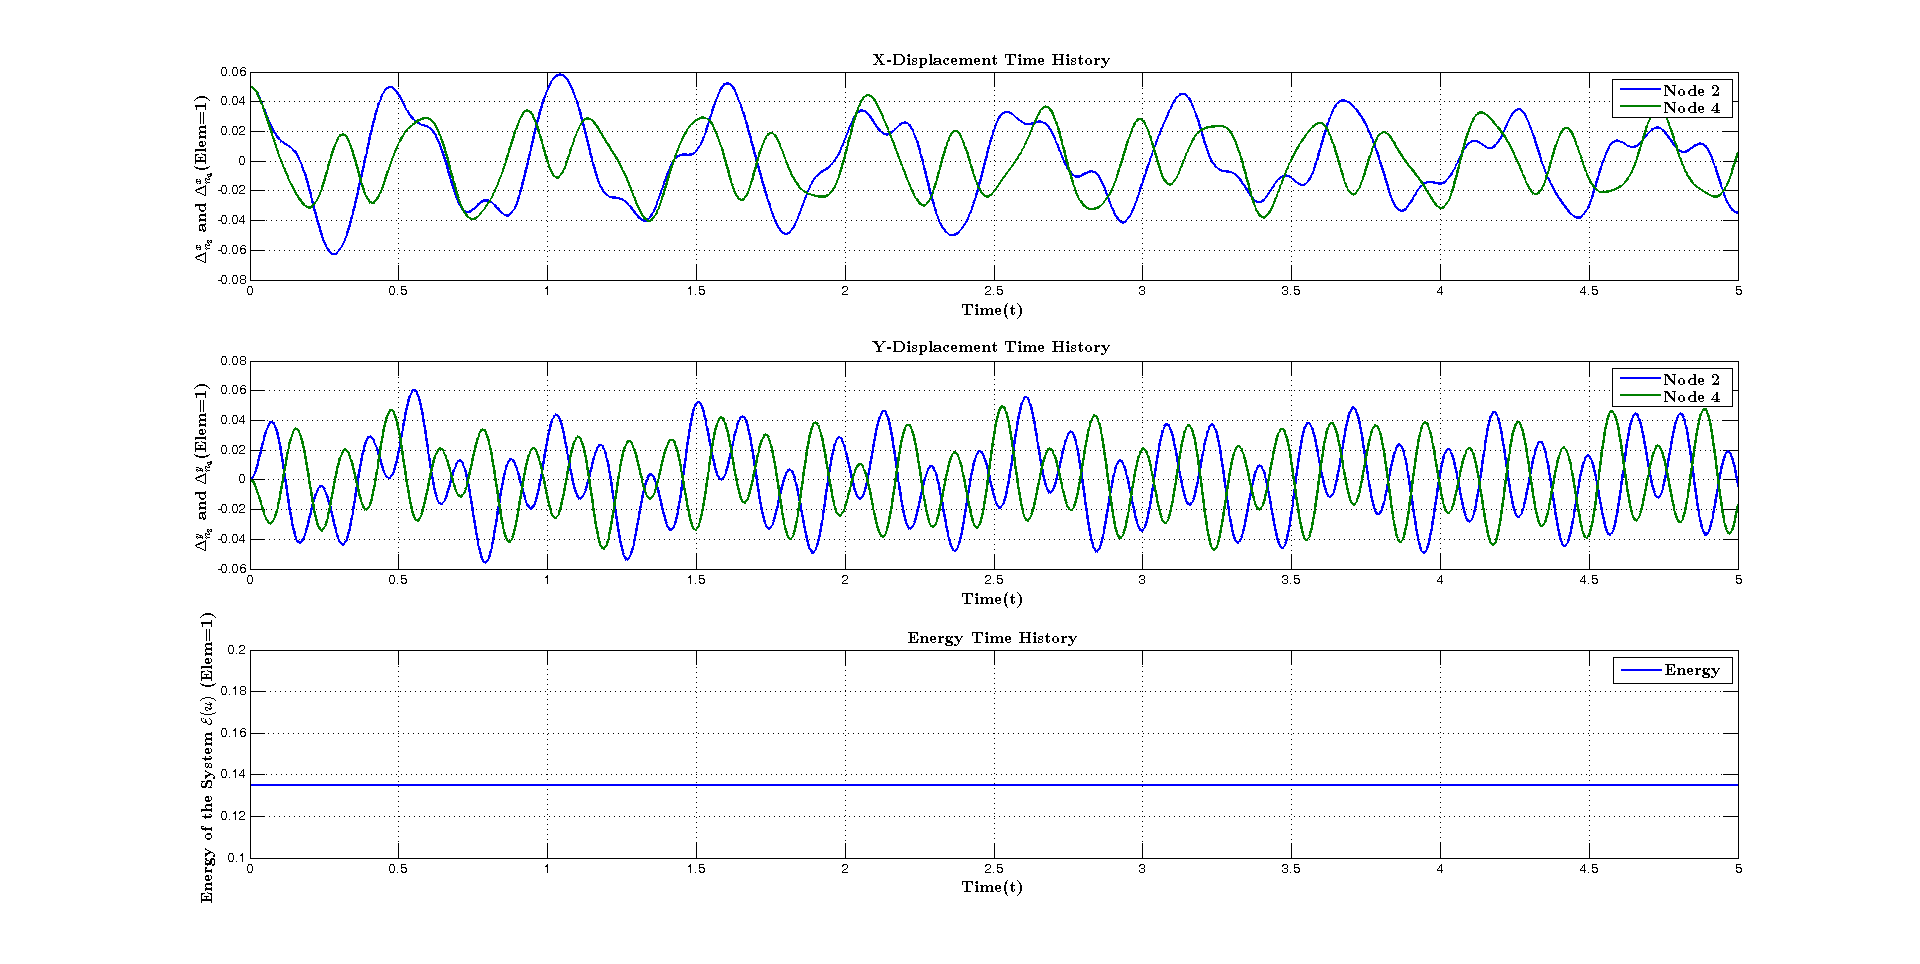
\includegraphics[height=5.5in,width=5.5in]{Disp_nobf_alphm1_3t3}
\end{center}\hrule